\documentclass{ximera}
\title{Analyzing Graphs and Piecewise Functions}

\outcome{Determine whether a function is even, odd, or neither from its formula.}
\outcome{Identify intervals of increase/decrease and relative extrema from a graph.}
\outcome{Evaluate and graph piecewise-defined functions.}
\outcome{Model real-world situations with piecewise functions.}

\begin{document}
\begin{abstract}
\end{abstract}
\maketitle

\textbf{Learning Objectives:}
\begin{itemize}
  \item Determine whether a function is even, odd, or neither from its formula.
  \item Identify intervals of increase/decrease and relative extrema from a graph.
  \item Evaluate and graph piecewise-defined functions.
  \item Model real-world situations with piecewise functions.
\end{itemize}
\medskip

\section*{Quick Check}

\begin{problem}
The piecewise graph below is shown.

\begin{center}
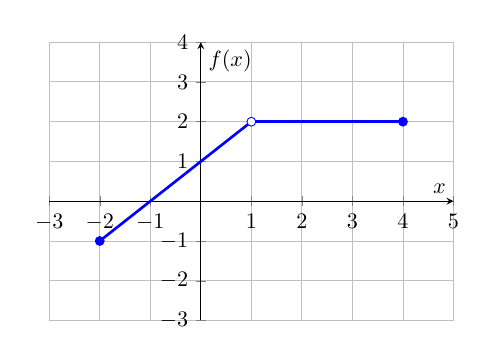
\begin{tikzpicture}[scale=0.8]
\begin{axis}[
  axis lines=middle,
  xmin=-3, xmax=5,
  ymin=-3, ymax=4,
  xtick={-3,...,5},
  ytick={-3,...,4},
  grid=both,
  width=8cm, height=6cm,
  xlabel={$x$}, ylabel={$f(x)$}
]
\addplot[very thick, blue, domain=-2:1] {x+1};
\addplot[very thick, blue, domain=1:4] {2};
\addplot[only marks, mark=*, mark options={fill=white}, blue] coordinates {(1,2)};
\addplot[only marks, mark=*, blue] coordinates {(-2,-1) (4,2)};
\end{axis}
\end{tikzpicture}
\end{center}

What is the value of $f(1)$?
\begin{hint}
Identify which branch, if any, includes $x = 1$ with a closed dot (filled circle).
\end{hint}
\begin{multipleChoice}
  \choice{$-1$}
  \choice{$0$}
  \choice{$1$}
  \choice{$2$}
  \choice[correct]{$f(1)$ is undefined}
\end{multipleChoice}
\end{problem}

\begin{problem}
Let $g(x) = \begin{cases} x^2 - 1 & x < 2 \\ 3x - 5 & x \geq 2 \end{cases}$. What is the domain of $g$?
\begin{hint}
The two branches together cover all real values of $x$.
\end{hint}
\begin{multipleChoice}
  \choice{$x < 2$}
  \choice{$x \leq 2$}
  \choice{$x \geq 2$}
  \choice{$(-\infty, 2]$}
  \choice[correct]{$(-\infty,\infty)$}
\end{multipleChoice}
\end{problem}

\begin{problem}
The graph of $h$ is shown.

\begin{center}
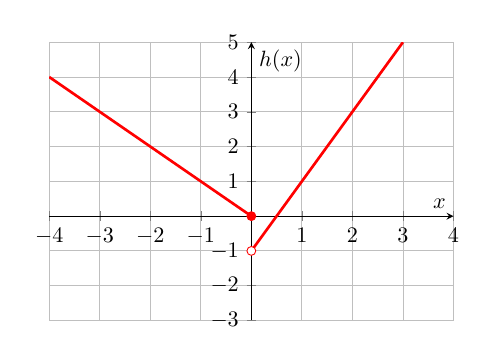
\begin{tikzpicture}[scale=0.8]
\begin{axis}[
  axis lines=middle,
  xmin=-4, xmax=4,
  ymin=-3, ymax=5,
  xtick={-4,...,4},
  ytick={-3,...,5},
  grid=both,
  width=8cm, height=6cm,
  xlabel={$x$}, ylabel={$h(x)$}
]
\addplot[very thick, red, domain=-4:0] {-x};
\addplot[very thick, red, domain=0:3] {2*x - 1};
\addplot[only marks, mark=*, red] coordinates {(0,0)};
\addplot[only marks, mark=*, mark options={fill=white}, red] coordinates {(0,-1)};
\end{axis}
\end{tikzpicture}
\end{center}

Which of the following defines $h(x)$?
\begin{hint}
Look at the slope of each branch and whether $x=0$ is included (closed) or excluded (open) in each branch.
\end{hint}
\begin{multipleChoice}
  \choice{$\begin{cases} x & x < 0 \\ 2x-1 & x \geq 0 \end{cases}$}
  \choice[correct]{$\begin{cases} -x & x \leq 0 \\ 2x-1 & x > 0 \end{cases}$}
  \choice{$\begin{cases} -x & x \leq 0 \\ 2x+1 & x > 0 \end{cases}$}
  \choice{$\begin{cases} x & x \leq 0 \\ 2x+1 & x > 0 \end{cases}$}
\end{multipleChoice}
\end{problem}

\begin{problem}
Let $f(x) = \begin{cases} x+2 & x < -1 \\ 3 & -1 \leq x \leq 2 \\ x-1 & x > 2 \end{cases}$. What is the range of $f$?
\begin{hint}
Determine the range of each branch separately, then take the union.
\end{hint}
\begin{multipleChoice}
  \choice{$(-\infty,\infty)$}
  \choice{$(-\infty,3]$}
  \choice{$(-\infty,3) \cup (1,\infty)$}
  \choice[correct]{$(-\infty,1) \cup \{3\} \cup (1,\infty)$}
  \choice{$(-\infty,1) \cup \{3\}$}
\end{multipleChoice}
\end{problem}

\begin{problem}
The graph of $f$ is shown and values of $g$ are given in the table.

\begin{center}
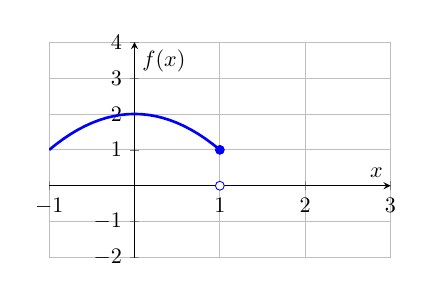
\begin{tikzpicture}[scale=0.8]
\begin{axis}[
  axis lines=middle,
  xmin=-1, xmax=3,
  ymin=-2, ymax=4,
  xtick={-1,...,3},
  ytick={-2,...,4},
  grid=both,
  width=7cm, height=5cm,
  xlabel={$x$}, ylabel={$f(x)$}
]
\addplot[very thick, blue, domain=-1:1] {-x^2 + 2};
\addplot[only marks, mark=*, blue] coordinates {(1,1)};
\addplot[only marks, mark=*, mark options={fill=white}, blue] coordinates {(1,0)};
\end{axis}
\end{tikzpicture}
\quad
\begin{tabular}{c|c}
$x$ & $g(x)$ \\\hline
2 & 3 \\
3 & 2 \\
4 & 0
\end{tabular}
\end{center}

Define $h(x) = \begin{cases} f(x) & x \leq 1 \\ g(x) & x > 1 \end{cases}$. Which gives the correct values of $h(1)$ and $h(3)$?
\begin{hint}
Use the branch condition to determine which function to apply for each input.
\end{hint}
\begin{multipleChoice}
  \choice{$h(1) = 0$, $h(3)$ is undefined}
  \choice{$h(1) = 0$, $h(3) = 3$}
  \choice{$h(1) = 1$, $h(3) = 3$}
  \choice{$h(1) = 0$, $h(3) = 2$}
  \choice[correct]{$h(1) = 1$, $h(3) = 2$}
\end{multipleChoice}
\end{problem}


\bigskip
\section*{Extended Practice}

\begin{problem}
Determine whether each function is even, odd, or neither from its graph. (Even functions are symmetric about the $y$-axis; odd functions have $180^\circ$ rotational symmetry about the origin.)
\begin{enumerate}
  \item[(a)]

\begin{center}
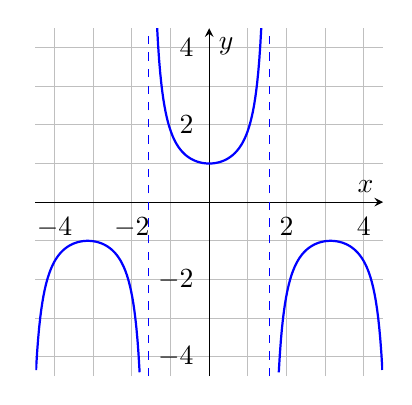
\begin{tikzpicture}
\begin{axis}[
  axis lines=center, width=6cm, height=6cm,
  xlabel={$x$}, ylabel={$y$},
  xmin=-4.5, xmax=4.5, xtick={-4,-2,0,2,4},
  ymin=-4.5, ymax=4.5, ytick={-4,-2,0,2,4},
  grid=both, minor tick num=1, tick style={draw=none},
]
\addplot[thick, blue, domain=-4.48:-1.8, samples=100] {1/cos(deg(x))};
\addplot[thick, blue, domain=-1.35:1.35, samples=100] {1/cos(deg(x))};
\addplot[thick, blue, domain=1.8:4.48, samples=100] {1/cos(deg(x))};
\addplot[dashed, thin, blue] coordinates {(-1.5708,-4.5) (-1.5708,4.5)};
\addplot[dashed, thin, blue] coordinates {(1.5708,-4.5) (1.5708,4.5)};
\end{axis}
\end{tikzpicture}
\end{center}

  \medskip
  \item[(b)]

\begin{center}
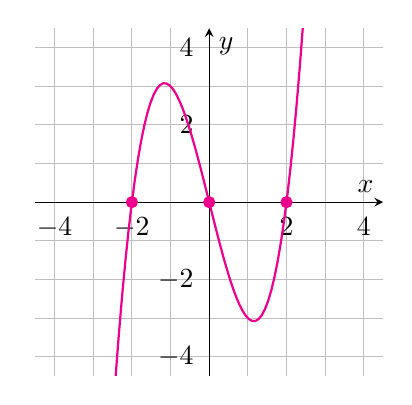
\begin{tikzpicture}
\begin{axis}[
  axis lines=center, width=6cm, height=6cm,
  xlabel={$x$}, ylabel={$y$},
  xmin=-4.5, xmax=4.5, xtick={-4,-2,0,2,4},
  ymin=-4.5, ymax=4.5, ytick={-4,-2,0,2,4},
  grid=both, minor tick num=1, tick style={draw=none},
]
\addplot[thick, magenta, domain=-2.42:2.43, samples=60] {x^3-4*x};
\addplot[only marks, mark=*, magenta] coordinates {(-2,0) (0,0) (2,0)};
\end{axis}
\end{tikzpicture}
\end{center}
\end{enumerate}

\begin{solution}
\begin{enumerate}
  \item[(a)] \textbf{Even} — the graph is symmetric about the $y$-axis.
  \item[(b)] \textbf{Odd} — the graph has $180^\circ$ rotational symmetry about the origin.
\end{enumerate}
\end{solution}
\end{problem}


\begin{problem}
Determine whether each function is even, odd, or neither. Justify your answer algebraically.
\begin{enumerate}
  \item[(a)] $p(x) = -|x| + 12x^{10} + 5$
  \medskip
  \item[(b)] $f(x) = \sqrt{81 - (x+2)^2}$
  \medskip
  \item[(c)] $\ds g(x) = \dfrac{-\sqrt[3]{x}}{x^2+1}$
  \medskip
  \item[(d)] $\ds h(x) = \dfrac{x^3}{2(x-1)^3}$
  \medskip
  \item[(e)] $k(x) = -x^8 + |3x|$
  \medskip
  \item[(f)] $a(x) = -8x^5 - 6x^3$
\end{enumerate}

\begin{solution}
\begin{enumerate}
  \item[(a)] $p(-x) = -|-x|+12(-x)^{10}+5 = -|x|+12x^{10}+5 = p(x)$. \textbf{Even.}

  \item[(b)] $f(-x) = \sqrt{81-(-x+2)^2} = \sqrt{81-(x-2)^2} \neq f(x)$ and $\neq -f(x)$. \textbf{Neither.}

  \item[(c)] $g(-x) = \dfrac{-\sqrt[3]{-x}}{(-x)^2+1} = \dfrac{\sqrt[3]{x}}{x^2+1} = -g(x)$. \textbf{Odd.}

  \item[(d)]
  \begin{align*}
    h(-x) &= \frac{(-x)^3}{2(-x-1)^3} = \frac{-x^3}{-2(x+1)^3} = \frac{x^3}{2(x+1)^3}
  \end{align*}
  This is not equal to $h(x)$ or $-h(x)$ (the denominator differs). \textbf{Neither.}

  \item[(e)] $k(-x) = -(-x)^8+|3(-x)| = -x^8+|3x| = k(x)$. \textbf{Even.}

  \item[(f)] $a(-x) = -8(-x)^5-6(-x)^3 = 8x^5+6x^3 = -(- 8x^5-6x^3) = -a(x)$. \textbf{Odd.}
\end{enumerate}
\end{solution}
\end{problem}


\begin{problem}
For each graph of $f(x)$ below, use interval notation to identify the intervals where $f$ is (i) increasing and (ii) decreasing, and (iii) state the location and value of any relative maxima or minima.

\begin{enumerate}
  \item[(a)]

\begin{center}
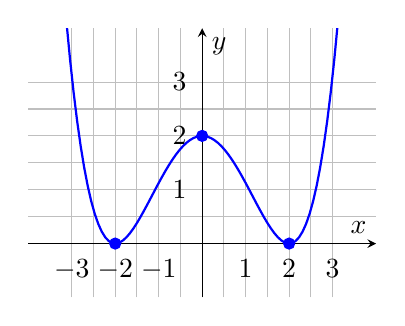
\begin{tikzpicture}
\begin{axis}[
  axis lines=center, width=6cm, height=5cm,
  xlabel={$x$}, ylabel={$y$},
  xmin=-4, xmax=4, xtick={-3,-2,-1,0,1,2,3},
  ymin=-1, ymax=4, ytick={0,1,2,3},
  grid=both, minor tick num=1, tick style={draw=none},
]
\addplot[thick, blue, domain=-3.2:3.2, samples=80] {x^4/8 - x^2 + 2};
\addplot[only marks, mark=*, blue] coordinates {(-2,0) (0,2) (2,0)};
\end{axis}
\end{tikzpicture}
\end{center}

  \medskip
  \item[(b)]

\begin{center}
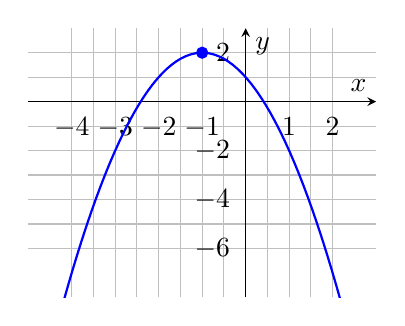
\begin{tikzpicture}
\begin{axis}[
  axis lines=center, width=6cm, height=5cm,
  xlabel={$x$}, ylabel={$y$},
  xmin=-5, xmax=3, xtick={-4,-3,-2,-1,0,1,2},
  ymin=-8, ymax=3, ytick={-6,-4,-2,0,2},
  grid=both, minor tick num=1, tick style={draw=none},
]
\addplot[thick, blue, domain=-4.2:2.2, samples=60] {-(x+1)^2 + 2};
\addplot[only marks, mark=*, blue] coordinates {(-1,2)};
\end{axis}
\end{tikzpicture}
\end{center}
\end{enumerate}

\begin{solution}
\begin{enumerate}
  \item[(a)]
  \begin{enumerate}
    \item[(i)] Increasing: $(-2,0)$ and $(2,\infty)$
    \item[(ii)] Decreasing: $(-\infty,-2)$ and $(0,2)$
    \item[(iii)] Relative maximum: $(0,2)$; Relative minima: $(-2,0)$ and $(2,0)$
  \end{enumerate}

  \item[(b)]
  \begin{enumerate}
    \item[(i)] Increasing: $(-\infty,-1)$
    \item[(ii)] Decreasing: $(-1,\infty)$
    \item[(iii)] No relative minimum; Relative maximum: $(-1,2)$
  \end{enumerate}
\end{enumerate}
\end{solution}
\end{problem}


\begin{problem}
Evaluate the functions at the indicated values.

\medskip
\textbf{(a)} $\ds f(x) = \begin{cases} 3, & -4 < x < -1\\ -x, & -1 \leq x < 3\\ \sqrt{x-3}, & x \geq 3 \end{cases}$

\begin{center}
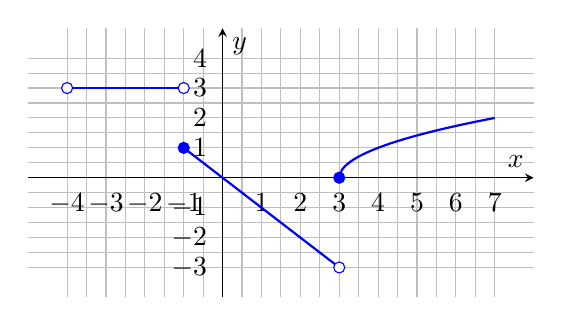
\begin{tikzpicture}
\begin{axis}[
  axis lines=center, width=8cm, height=5cm,
  xlabel={$x$}, ylabel={$y$},
  xmin=-5, xmax=8, xtick={-4,-3,-2,-1,0,1,2,3,4,5,6,7},
  ymin=-4, ymax=5, ytick={-3,-2,-1,0,1,2,3,4},
  grid=both, minor tick num=1, tick style={draw=none},
]
% Branch 1: y=3 for (-4,-1), open at both ends
\addplot[thick, blue, domain=-4:-1] {3};
\addplot[only marks, mark=*, mark options={fill=white}, blue] coordinates {(-4,3) (-1,3)};
% Branch 2: y=-x for [-1,3), closed at -1, open at 3
\addplot[thick, blue, domain=-1:3] {-x};
\addplot[only marks, mark=*, mark options={fill=white}, blue] coordinates {(3,-3)};
\addplot[only marks, mark=*, blue] coordinates {(-1,1)};
% Branch 3: y=sqrt(x-3) for x>=3, closed at (3,0)
\addplot[thick, blue, domain=3:7, samples=60] {sqrt(x-3)};
\addplot[only marks, mark=*, blue] coordinates {(3,0)};
\end{axis}
\end{tikzpicture}
\end{center}

\begin{enumerate}
  \item[(i)] $f(-3)$
  \medskip
  \item[(ii)] $f(-1)$
  \medskip
  \item[(iii)] $f(3)$
  \medskip
  \item[(iv)] $f(4)$
\end{enumerate}

\medskip
\textbf{(b)} $\ds g(x) = \begin{cases} -3x+1, & x < -1 \\ x^2-2, & -1 \leq x < 2\\ 5, & x \geq 2 \end{cases}$

\begin{center}
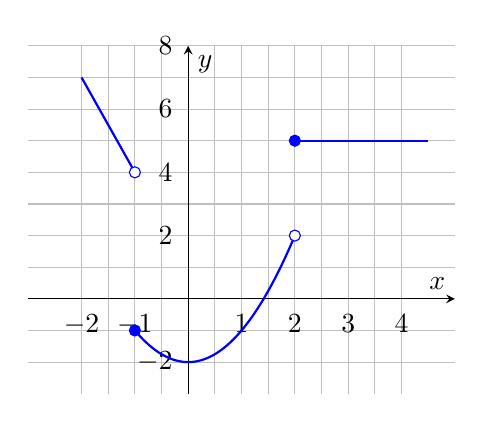
\begin{tikzpicture}
\begin{axis}[
  axis lines=center, width=7cm, height=6cm,
  xlabel={$x$}, ylabel={$y$},
  xmin=-3, xmax=5, xtick={-2,-1,0,1,2,3,4},
  ymin=-3, ymax=8, ytick={-2,0,2,4,6,8},
  grid=both, minor tick num=1, tick style={draw=none},
]
% Branch 1: y=-3x+1 for x<-1, show from x=-2
\addplot[thick, blue, domain=-2:-1] {-3*x+1};
\addplot[only marks, mark=*, mark options={fill=white}, blue] coordinates {(-1,4)};
% Branch 2: y=x^2-2 for -1<=x<2, closed at -1, open at 2
\addplot[thick, blue, domain=-1:2, samples=60] {x^2-2};
\addplot[only marks, mark=*, mark options={fill=white}, blue] coordinates {(2,2)};
\addplot[only marks, mark=*, blue] coordinates {(-1,-1)};
% Branch 3: y=5 for x>=2, closed at 2
\addplot[thick, blue, domain=2:4.5] {5};
\addplot[only marks, mark=*, blue] coordinates {(2,5)};
\end{axis}
\end{tikzpicture}
\end{center}

\begin{enumerate}
  \item[(i)] $g(-2)$
  \medskip
  \item[(ii)] $g(-1)$
  \medskip
  \item[(iii)] $g(2)$
  \medskip
  \item[(iv)] $g(5)$
\end{enumerate}

\begin{solution}
\textbf{(a)}
\begin{enumerate}
  \item[(i)] $f(-3) = 3$ (since $-4 < -3 < -1$)
  \item[(ii)] $f(-1) = -(-1) = 1$ (since $-1 \leq -1 < 3$)
  \item[(iii)] $f(3) = \sqrt{3-3} = 0$ (since $3 \geq 3$)
  \item[(iv)] $f(4) = \sqrt{4-3} = 1$ (since $4 \geq 3$)
\end{enumerate}

\medskip
\textbf{(b)}
\begin{enumerate}
  \item[(i)] $g(-2) = -3(-2)+1 = 7$ (since $-2 < -1$)
  \item[(ii)] $g(-1) = (-1)^2-2 = -1$ (since $-1 \leq -1 < 2$)
  \item[(iii)] $g(2) = 5$ (since $2 \geq 2$)
  \item[(iv)] $g(5) = 5$ (since $5 \geq 2$)
\end{enumerate}
\end{solution}
\end{problem}


\begin{problem}
A cell phone plan charges \$49.95/month plus \$14.02 in taxes, plus \$0.40/min for calls beyond a 600-minute monthly limit. Write a piecewise-defined function $C(x)$ modeling the monthly cost (in \$) as a function of the number of minutes used $x$.

\begin{solution}
The flat monthly cost is $\$49.95 + \$14.02 = \$63.97$.
$$C(x) = \begin{cases} 63.97, & 0 \leq x \leq 600\\ 63.97 + 0.4(x-600), & x > 600 \end{cases}$$
The term $(x-600)$ charges only the minutes \textit{beyond} the 600-minute included limit.
\end{solution}
\end{problem}


\begin{problem}
\textbf{Challenge.} Write a piecewise-defined function $f(x)$ for each graph shown below.
\begin{enumerate}
  \item[(a)]

\begin{center}
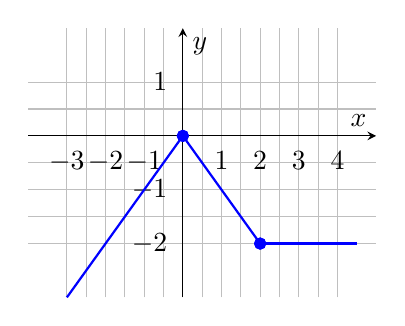
\begin{tikzpicture}
\begin{axis}[
  axis lines=center, width=6cm, height=5cm,
  xlabel={$x$}, ylabel={$y$},
  xmin=-4, xmax=5, xtick={-3,-2,-1,0,1,2,3,4},
  ymin=-3, ymax=2, ytick={-2,-1,0,1},
  grid=both, minor tick num=1, tick style={draw=none},
]
% Branch 1: y=x for x<=0 (slope 1, closed at origin)
\addplot[thick, blue, domain=-3:0] {x};
% Branch 2: y=-x for 0<x<=2 (slope -1)
\addplot[thick, blue, domain=0:2] {-x};
% Branch 3: y=-2 for x>2
\addplot[thick, blue, domain=2:4.5] {-2};
% Open dots first
\addplot[only marks, mark=*, mark options={fill=white}, blue] coordinates {(0,0) (2,-2)};
% Closed dots (branch 1 at origin, branch 2 at x=2)
\addplot[only marks, mark=*, blue] coordinates {(0,0) (2,-2)};
\end{axis}
\end{tikzpicture}
\end{center}

  \medskip
  \item[(b)]

\begin{center}
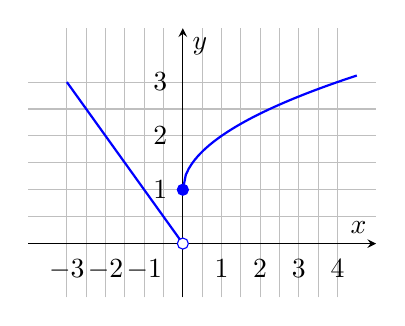
\begin{tikzpicture}
\begin{axis}[
  axis lines=center, width=6cm, height=5cm,
  xlabel={$x$}, ylabel={$y$},
  xmin=-4, xmax=5, xtick={-3,-2,-1,0,1,2,3,4},
  ymin=-1, ymax=4, ytick={0,1,2,3},
  grid=both, minor tick num=1, tick style={draw=none},
]
% Branch 1: y=-x for x<0 (slope -1, open at origin)
\addplot[thick, blue, domain=-3:0] {-x};
\addplot[only marks, mark=*, mark options={fill=white}, blue] coordinates {(0,0)};
% Branch 2: y=sqrt(x)+1 for x>=0 (closed at (0,1))
\addplot[thick, blue, domain=0:4.5, samples=60] {sqrt(x)+1};
\addplot[only marks, mark=*, blue] coordinates {(0,1)};
\end{axis}
\end{tikzpicture}
\end{center}
\end{enumerate}

\begin{solution}
\begin{enumerate}
  \item[(a)] $$f(x) = \begin{cases} x, & x \leq 0\\ -x, & 0 < x \leq 2\\ -2, & x > 2 \end{cases}$$
  (Alternatively: $f(x) = \begin{cases} -|x| & x \leq 2\\ -2 & x > 2 \end{cases}$)

  \item[(b)] $$f(x) = \begin{cases} -x, & x < 0\\ \sqrt{x}+1, & x \geq 0 \end{cases}$$
\end{enumerate}
\end{solution}
\end{problem}

\end{document}
